\newcommand{\FigBentSolenoidRelativeDrift}{
\begin{figure}[t]
\centering
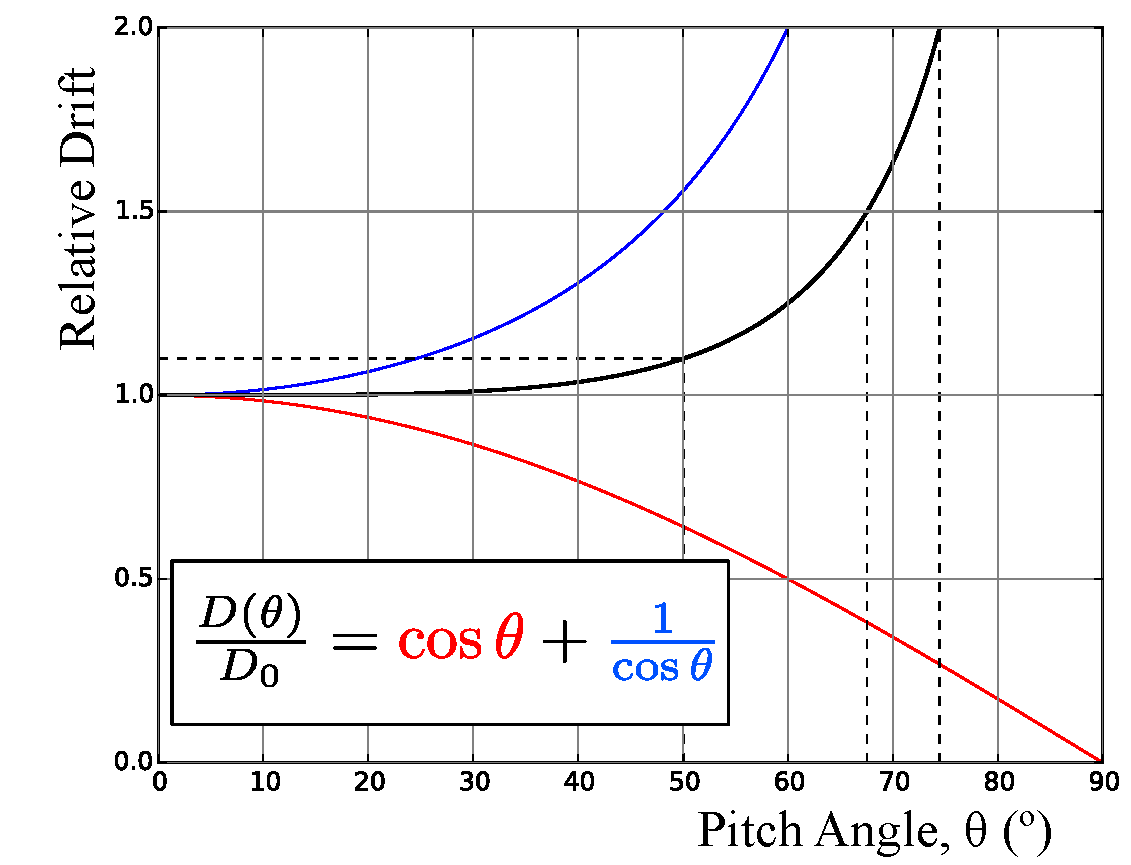
\includegraphics[width=0.6\textwidth]{figs/detector/BentSolenoids_RelativeDrift}
\caption{
Angular dependence of the magnitude of vertical drift in a bent solenoid field.
The total variation (black) remains below 10\% for pitch angles below 50\degree.
}
\figlabel{detector:bent-solenoids:angularDependence}
\end{figure}
}

\newcommand{\FigPhaseII}{
\begin{figure}[t]
\centering
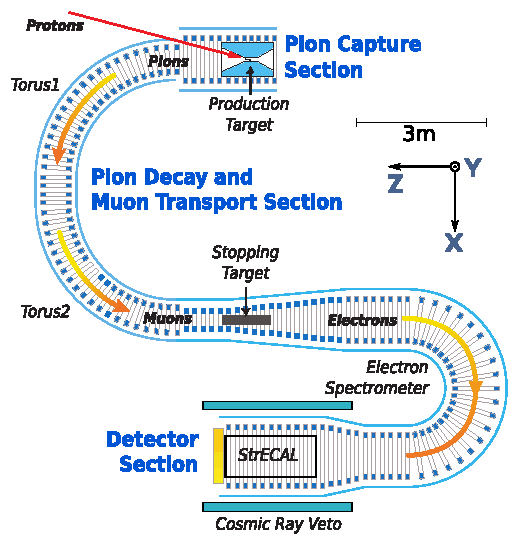
\includegraphics[width=0.9\textwidth]{figs/detector/PhaseII_schematic}
\caption{
Schematic layout of COMET \phaseII. 
The 8 GeV proton beam enters from the top-left, producing (amongst other things) pions.
Pions and muons travelling backwards with respect to the proton beam are then transported around 180 degrees of bent solenoid, during which time most of the pions decay producing an intense muon beam.
About 40\% of these muons then stop in the stopping target (centre of image).
Any electrons coming from  \mueconv are then transported through another 180 degrees of bent solenoid into the detector system.
}
\figlabel{detector:PhaseII:setup}
\end{figure}
}

\newcommand{\FigPhaseI}{
\begin{figure}[t]
\centering
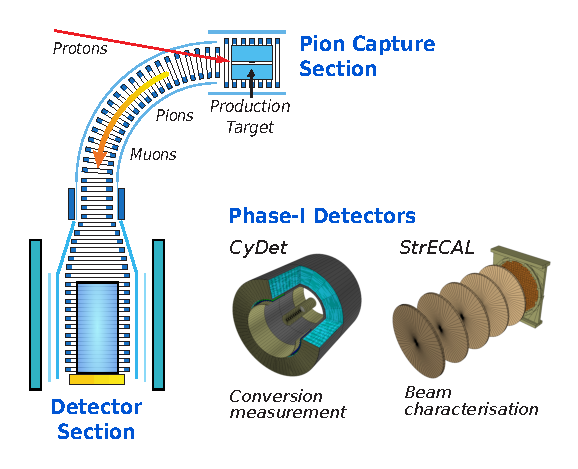
\includegraphics[height=0.4\textheight]{figs/detector/PhaseI_schematic}
\caption{
Schematic layout of COMET \phaseI. 
}
\figlabel{detector:PhaseI:setup}
\end{figure}
}

\newcommand{\TabBackgroundSummary}{
\begin{table}
\begin{tabular}{lldd}
     \hline
     \hline\\[-1.8ex]
     Type           & Background & \multicolumn{2}{c}{Predicted number of events during run} \\
                    &  & \multicolumn{1}{c}{\phaseI \cite{TDR2014}} & \multicolumn{1}{c}{\phaseII \cite{CDRphase2} } \\
     \hline\\[-1.8ex]
     Intrinsic & Muon Decay-in-Orbit                       & 0.01              & 0.15    \\
               & Radiative Muon Capture                    & 0.00056           & <0.001  \\
               & $\mu^-$ Capture w/ n Emission             & <0.001            & <0.001  \\
               & $\mu^-$ Capture w/ Charged Part. Emission & <0.001            & <0.001  \\
     Prompt    & Radiative Pion Capture                    & 0.00023           & 0.05    \\
               & Beam Electrons                            & 0.00083           & <0.1^*  \\
               & Muon Decay in Flight                      & \le0.0002         & <0.0002 \\
               & Pion Decay in Flight                      & \le0.00023        & <0.0001 \\
               & Neutron Induced                           & -                 & 0.024   \\
               & Other beam induced B.G.                   & <2.8\times10^{-6} & -       \\
     Delayed   & Delayed Radiative Pion Capture            & \sim0             & 0.002   \\
               & Anti-proton Induced                        & 0.007             & 0.007   \\
               & Other delayed B.G.                        & \sim0             & -       \\
     Cosmic    & Cosmic Ray Muons                          & -                 & 0.002   \\
               & Electrons from Cosmic Ray Muons           & <0.0001           & 0.002   \\
     \hline\\[-1.8ex]
     \multicolumn{2}{c}{Total background}                      & 0.019         & 0.34    \\
     \multicolumn{2}{c}{Signal (Assuming $B=1\times10^{-16}$)} & 0.31          & 3.8     \\
     \hline
     \hline
\end{tabular}
\caption{
	\CHECK{UPDATE \phaseI values with TDR 2016}
	Backgrounds for COMET \phaseI \cite{TDR2014} and \phaseII \cite{CDRphase2}.
	Prompt backgrounds arise by protons that occur in between bunches and are therefore suppressed by the extinction factor.
	For \phaseI, the recently measured value of $10^{-12}$ was used for the extinction factor, but for \phaseII the older expectation of $10^{-9}$ was used.
}
\tablabel{detector:backgrounds}
\end{table}
}

\newcommand{\FigMuonNuclearParams}{
\begin{figure}[bp]
\centering
\subfloat[][\figlabel{detector:mu-nucl-params:lifetimes}Lifetimes]{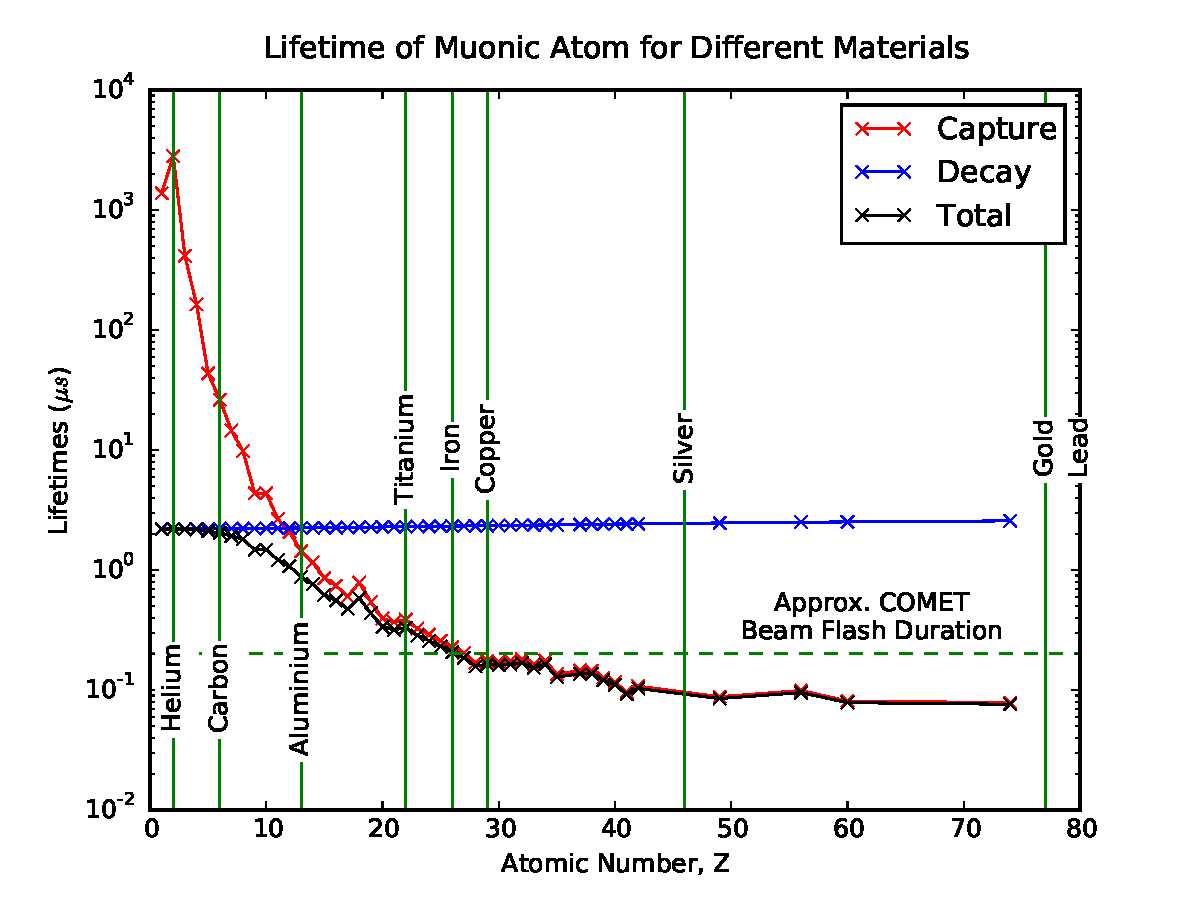
\includegraphics[width=0.9\textwidth]{figs/detector/MuNuclearParams_All_lifetimes.pdf}}\\
\subfloat[][\figlabel{detector:mu-nucl-params:end-point}End-point Shift]{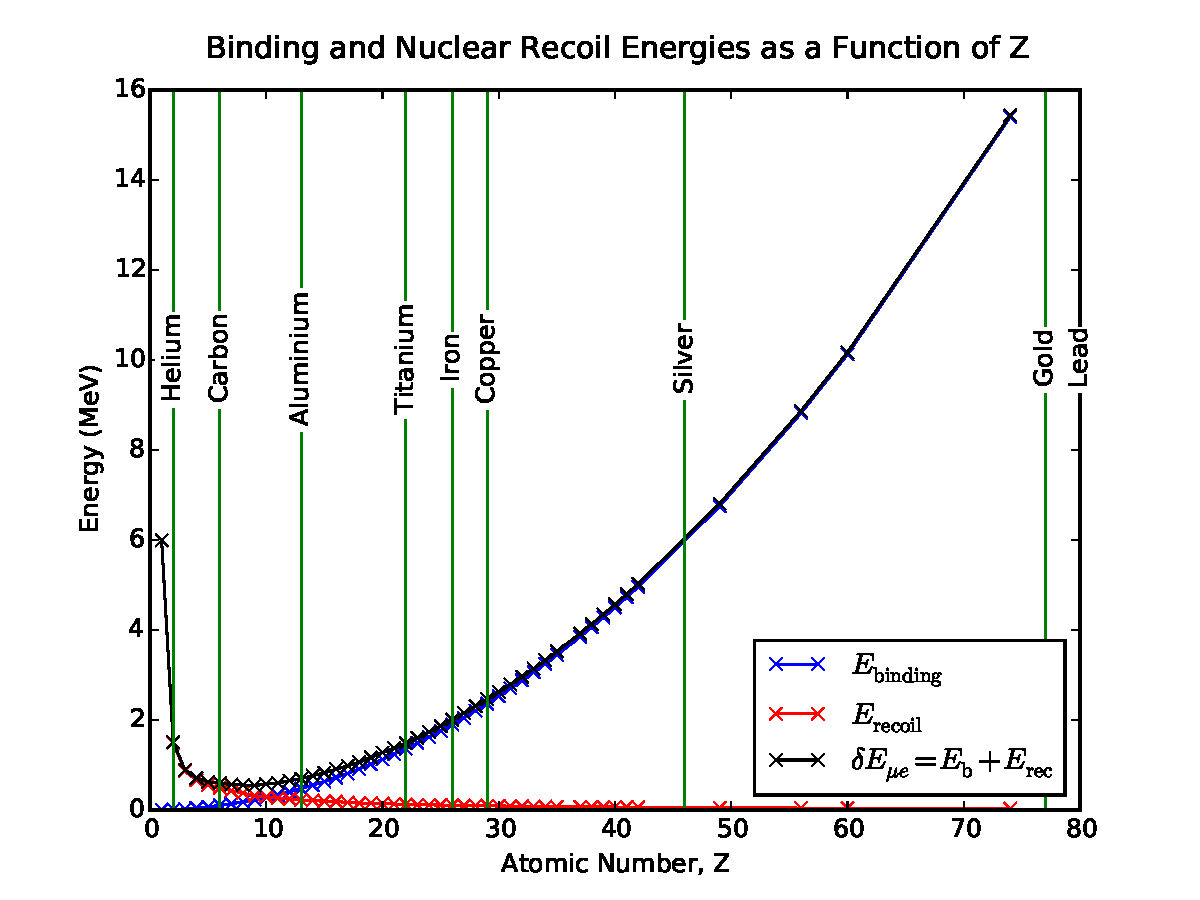
\includegraphics[width=0.49\textwidth]{figs/detector/MuNuclearParams_energies.pdf}}%\hspace{0.5cm}%
\subfloat[][\figlabel{detector:mu-nucl-params:branching-ratio}Branching Fraction]{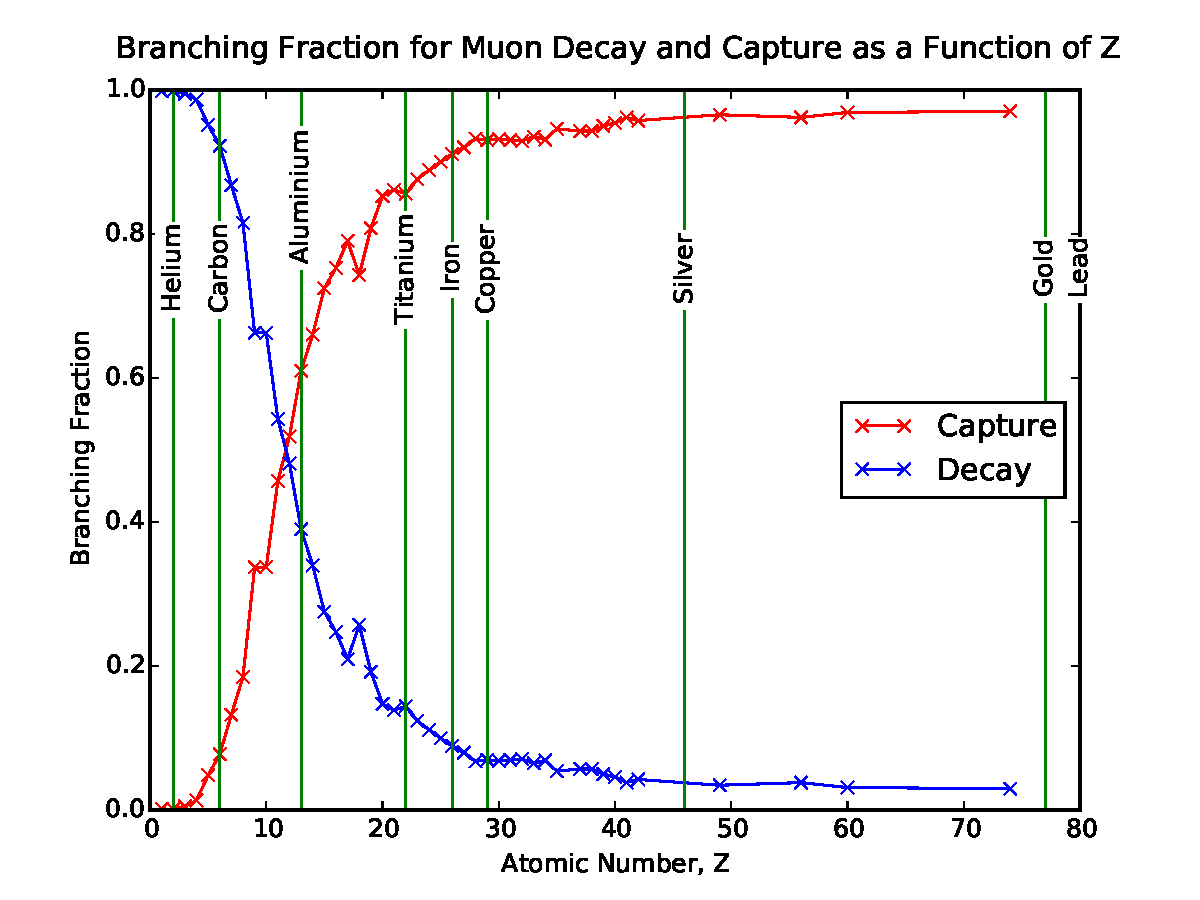
\includegraphics[width=0.49\textwidth]{figs/detector/MuNuclearParams_branching_fraction.pdf}}
\caption{\figlabel{detector:mu-nucl-params}
The effect of changing the atomic number on the branching ratio, lifetime and electron energy spectrum end-point.
For the branching ratio and lifetime plots, the partial rate for muon nuclear capture and decay-in-orbit are shown separately.
The capture and decay rates are taken from the Geant4 \cite{Geant42003} parametrisation for stopped negative muons.  
Only elements for which at least 1 isotope uses a measured value are plotted.
The values for the end-point energy level are calculated using the Bohr model for the muon ground-state binding energy.
}
\end{figure}
}
